%
% For LaTeXML: 
% latexml Differentiation\ 1.tex --dest=Diff1.xml
% latexmlpost Diff1.xml --dest=Differentiation\ 1.html --split --splitat=section --navigationtoc=context --javascript="https://cdn.jsdelivr.net/npm/mathjax@3/es5/tex-mml-chtml.js?config=MML_HTMLorMML" --urlstyle=file --timestamp=0
%
%%
\documentclass[12pt]{article}
\title{\vspace{-1.5cm} Differentiation 1 \vspace{-1.5cm}}
\date{}
\usepackage{fancyhdr,amsmath,amssymb,amsthm,graphicx,float,enumerate,parskip,latexml}

\iflatexml
\newenvironment{shaded}[1][]{
}
\else
\usepackage{tikz,framed}
\definecolor{shadecolor}{HTML}{F2F2F2} % for framed
\usepackage[hide links]{hyperref}
\fi

\theoremstyle{definition} % Easier to read than \theoremstyle{example} --- no italics
\newtheorem{mydef}{Definition}
\newtheorem{eg}[mydef]{Example}
\newtheorem{ex}[mydef]{Exercise}
\newtheorem*{sol}{Solution}
\usepackage[margin=2.5cm,top=2cm,bottom=5cm]{geometry}
%\usepackage[a4paper,left=1.27cm,right=1.27cm,bottom=5cm,]{geometry}
\pagestyle{empty} % For headers and footers on first page only. Change to \pagestyle{fancy} for headers and footers on every page.
\fancyhf{}
\renewcommand{\headrulewidth}{0pt} 
\fancyfoot[C]{\vspace*{1pt} % Adds a little vertical space
   
\includegraphics[width=3cm]{UoS.jpg}\hfill
\includegraphics[width=1cm]{301.png}\hfill
\includegraphics[width=1.25cm]{MASH.png} % Logos
}
\fancyhead[L]{\tiny{Author: Rosie Shewell Brockway}}	% Author
\fancyhead[R]{\tiny{Date created: 05/02/2021 \\ Updated: 21/11/2022}} % Date
%


\renewcommand{\familydefault}{\sfdefault} %This makes everything apart from equations sans serif for readability
\usepackage[default]{sourcesanspro}
\usepackage[T1]{fontenc}


\begin{document}
\setlength{\headheight}{1cm}
\maketitle
\thispagestyle{fancy} % For headers and footers on first page only.


Differentiation is a method for calculating the gradient of a curve at a given point. On this sheet, we recap the definition of the derivative of a function in one variable and practice the method of differentiation from first principles. 

We will also revise the standard formula for the derivative of a power, and practice using it to differentiate polynomials. The problem set at the end of this resource includes some contextual questions to give a taste of how differentiation can be used to solve problems in the real world.

\subsection*{First Principles Differentiation}

\begin{shaded}
\begin{mydef}
The derivative of a function $f$ at a point $P=(a,f(a))$ on the curve $y=f(x)$ is
	\begin{equation}\label{eq:f'(a)}
	f'(a) = \lim_{h\rightarrow 0}\frac{f(a+h)-f(a)}{h}.
	\end{equation}
\end{mydef}
\end{shaded}

The rationale for this formula is the following: suppose $Q$ is a second point on the curve, very close to $P$. 

\begin{figure}[H]
\centering
\iflatexml
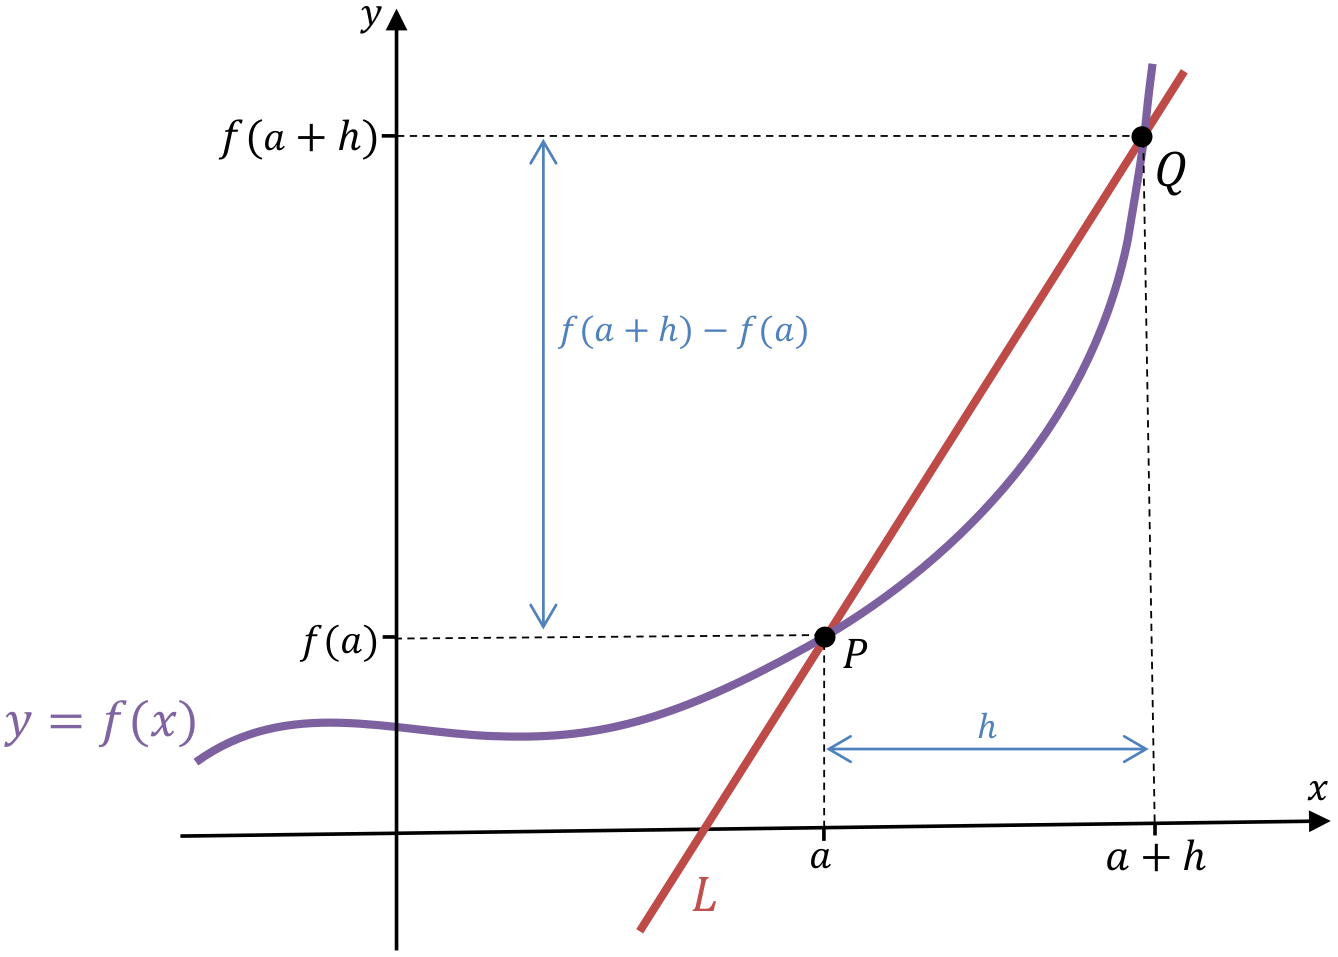
\includegraphics[width=1\linewidth]{f'(a)}
\else
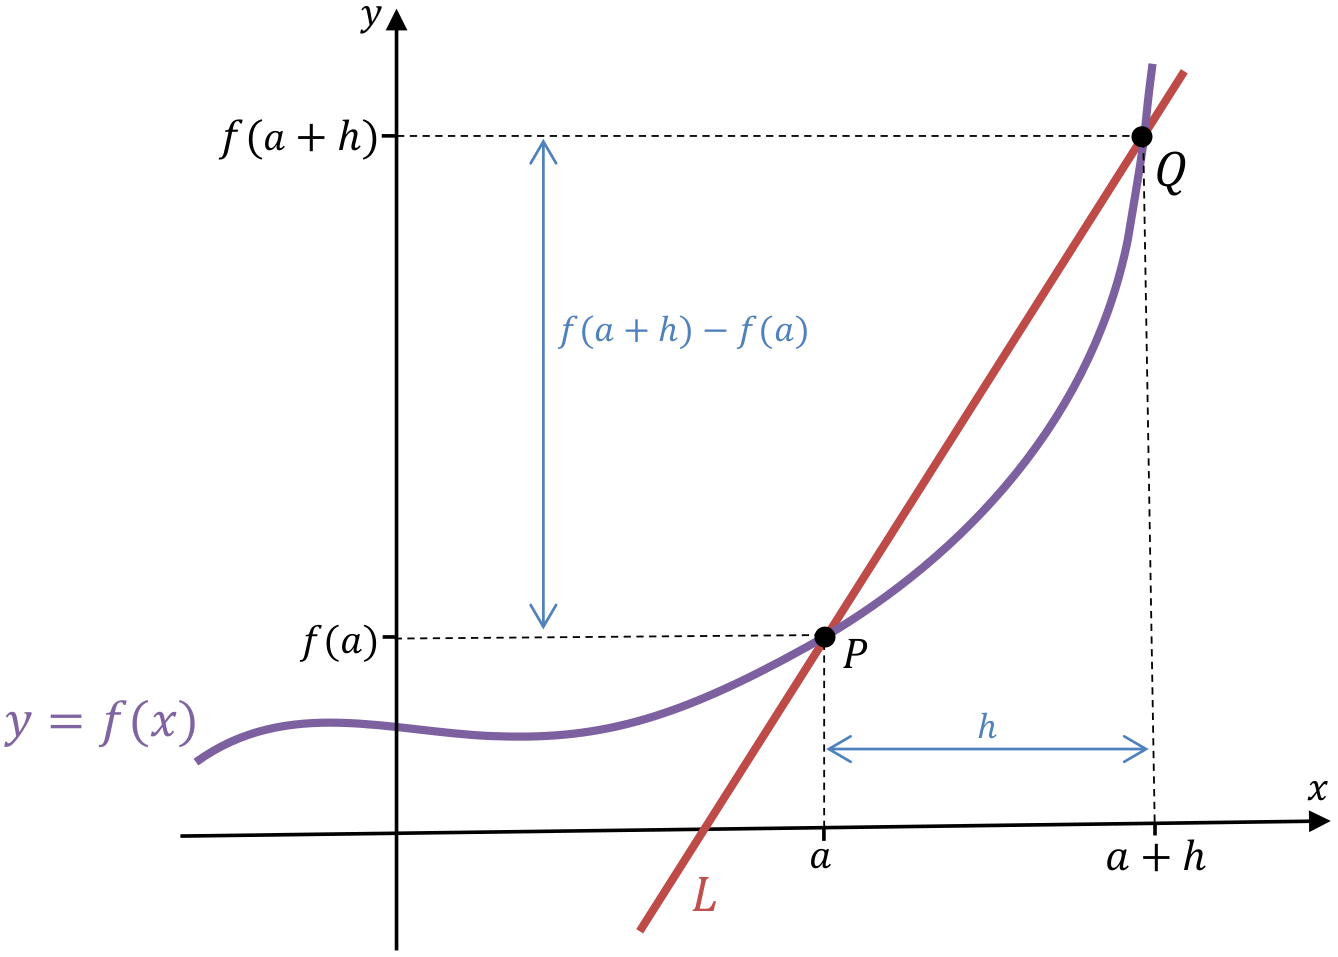
\includegraphics[width=.65\linewidth] {f'(a)} 
\fi
\caption{Two nearby points on a curve, connected by a straight line.}
\end{figure}

Provided $P$ and $Q$ are very close together, the line $L$ passing through both of these points will give a good approximation for the tangent line at $P$.

Suppose that $P=(a,f(a))$ and $Q = (a+h,f(a+h))$, where $h$ is a very small number.

The gradient of the straight line through $P$ and $Q$ is given by the standard formula
	\[\text{Gradient of } L = \frac{\text{Change in }y}{\text{Change in }x} = \frac{f(a+h)-f(a)}{h}\]
As $h$ becomes very small, the point $Q$ approaches $P$, and $L$ becomes the tangent line at $P$. The gradient of $L$ becomes the derivative of $f$ at $P$, given by formula (\ref{eq:f'(a)}). 

Differentiation using (\ref{eq:f'(a)}) is sometimes called \emph{differentiation by first principles}.

Since we want to view the derivative as a funciton, we tend to use $x$ instead of $a$ in formula (\ref{eq:f'(a)}). Then, the derivative is given by
	\begin{equation}\label{eq:f'(x)}
	f'(x) = \lim_{h\rightarrow 0}\frac{f(x+h)-f(x)}{h}
	\end{equation}

\begin{eg}
Differentiate $f(x)=3x^2$ from first principles.
\end{eg}
\begin{sol}
We use (\ref{eq:f'(x)}). Before we can evaluate the limit, we calculate $\frac{f(x+h)-f(x)}{h}$ for this particular function $f(x)=3x^2$.

We have
	\begin{align*}
	\frac{f(x+h)-f(x)}{h} &= \frac{3(x+h)^2-3x^2}{h} \\
	&= \frac{3(x^2+2xh+h^2)-3x^2}{h} \\
	&= \frac{3x^2 + 6xh + 3h^2 -3x^2}{h} \\
	&=\frac{6xh+3h^2}{h} = 6x+3h.
	\end{align*}
Letting $h$ tend to zero, we then get
	\[f'(x) = \lim_{h\rightarrow 0}\frac{f(x+h)-f(x)}{h} = \lim_{h\rightarrow 0}(6x+h) = 6x.\]
\end{sol}

\begin{ex}\label{ex:1stprinciples}
Let $f(x)=x^3$.
\begin{enumerate}[(i)]
\item Calculate $\displaystyle\frac{f(x+h)-f(x)}{h}$.
\item Hence use (\ref{eq:f'(x)}) to differentiate $f(x)$ from first principles.
\end{enumerate}
\end{ex}

\subsection*{Some Properties of Derivatives}
\subsubsection*{Linearity Property}
\begin{shaded}
If two functions $f(x)$ and $g(x)$ are differentiable, and $a$ and $b$ are constants, then the derivative of $af(x)+bg(x)$ is
	\[\frac{d}{dx}\left(af(x)+bg(x)\right) = af'(x) + bg'(x).\]
\end{shaded}

\subsubsection*{Differentiating Powers}
\begin{shaded}
\noindent{\bf General rule:} For any non-zero real number $r$,
	\begin{equation}\label{eq:diffpowers}
	\frac{d}{dx}\left(x^r\right) = rx^{r-1}.
	\end{equation} 
\end{shaded}

Equation (\ref{eq:diffpowers}) may be used in conjunction with the linearity property for derivatives to differentiate any linear combination of powers of $x^r$.

\begin{eg}
Use equation (\ref{eq:diffpowers}) to differentiate $f(x)=3x^2-2\sqrt{x}+\frac{7}{x^3}$.
\end{eg}
\begin{sol}
First we rewrite the expression for $f(x)$ using power notation:
	\[f(x)=3x^2 -3x^{\frac{1}{2}} + 7x^{-3}.\]
By the linearity property for derivatives, we can calculate $f'(x)$ by differentiating term by term. Each term can be differentiating using the power rule (\ref{eq:diffpowers}). Hence
	\begin{align*}
	f'(x) &= 6x - 3\cdot\frac{1}{2}x^{-\frac{1}{2}}+7(-3)x^{-4} \\
	&= 6x - \frac{3}{2\sqrt{x}}-\frac{21}{x^4}.
	\end{align*} 
\end{sol}

\begin{ex}\label{ex:diffpowers}
Use (\ref{eq:diffpowers}) to differentiate $\displaystyle 15x-\frac{2}{\sqrt[3]{x}}-\frac{x^4}{2}$ with respect to $x$.
\end{ex}


%\iflatexml
%\begin{center}
%\vspace*{1pt} % Adds a little vertical space
%\begin{tabular}{lcccr}
%   
\includegraphics[width=3cm]{UoS.jpg} & \includegraphics[width=10cm]{blank.png}  &
\includegraphics[width=1cm]{301.png} & \includegraphics[width=10cm]{blank.png}  & 
\includegraphics[width=1.25cm]{MASH.png} % Logos
%\end{tabular}
%\end{center}
%\else
%\fi

\newpage

\section*{Solutions to Exercises}
\noindent{\bf Solution to Exercise \ref{ex:1stprinciples}:} 
\begin{enumerate}[(i)]
\item We have $f(x)=x^3$, and so
	\begin{align*}
	\frac{f(x+h)-f(x)}{h} &= \frac{(x+h)^3 - x^3}{h} \\
	&= \frac{x^3 + 3hx^2 + 3h^2x + h^3 - x^3}{h} \\
	&= \frac{3hx^2++3h^2x+h^3}{h} = 3x^2 +3hx +h^2
	\end{align*}
\item Hence 
	\[f'(x) = \lim_{h\rightarrow 0}\left(3x^2 +3hx +h^2\right)=3x^2.\]
\end{enumerate}

\noindent{\bf Solution to Exercise \ref{ex:diffpowers}:} 
	\begin{align*}
	\frac{d}{dx}\left( 15x-\frac{2}{\sqrt[3]{x}}-\frac{x^4}{2} \right) &= \frac{d}{dx}\left( 15x-2x^{\frac{1}{3}}-\frac{1}{2}x^4\right) \\
	&=15-2\cdot\frac{1}{3}x^{-\frac{2}{3}}-\frac{1}{2}\cdot 4x^3 = 15-\frac{2}{3}x^{-\frac{2}{3}}-2x^3.
	\end{align*} 
	
\end{document}
